% --*- coding:utf-8-unix mode:latex -*--
%\include{begin}
%%%%%%%%%%%%%%%%%%%%%%%%%%%%%%%%%%%%%%%%%%%%%%%%%%%%%%%%%%%%%%%%%%%%%%%%%%%%%%%

\section{退所式}

\subsection{日時・場所}
\begin{tabular}{p{2zw}rp{38zw}}
  日時 & : & 2019年4月6日(土) 11:25 $\sim$ 11:55\\
  場所 & : & 体育館
\end{tabular}

\subsection{タイムスケジュール}
% 時刻は必ず4桁(00:00)で書くこと!!!
\begin{longtable}{p{3zw}p{39zw}}
  11:25 & \textbf{◎ トイレ休憩} \\
        & \ \ \textbullet \ \ 司会(生野,貞松)はトイレ休憩のアナウンスを行う\\
        & \ \ \textbullet \ \ ペーパードミノの点数集計結果を小島に伝え,小島がパワーポイントに反映する\\
        & \ \ \textbullet \ \ 司会者は整列をするように促す\\
        & \ \ \textbullet \ \ 各班のスタッフはプラカードを持ち一列に整列させ,全員が揃った班はその場に座る \\\\
        & \ \ \textbullet \ \ 日下は幡多職員に退所挨拶のお願いと記念撮影のお願いをするために,事務室に行く \\\\

  11:40 & \textbf{◎ Flying Fish斉唱} \\
  	& \ \ \textbullet \ \ 小島はFlying Fishを流す \\\\

  11:46 & \textbf{◎ 代表挨拶)} \\
	& \ \ \textbullet \ \ 司会は代表(宮尾)にマイクを渡す \\\\

  11:48 & \textbf{◎ 幡多職員による挨拶} \\
  	& \ \ \textbullet \ \ 宮尾は幡多職員にマイクを渡す \\
  	& \ \ \textbullet \ \ 挨拶が終わり次第,宮尾はマイクを受け取る \\\\

  11:50 & \textbf{◎ 記念撮影} \\
	& \ \ \textbullet \ \ 幡多職員に記念撮影を行ってもらう \\
        & \ \ \textbullet \ \ 体育館の2階から撮影し,司会(もしくは近くのスタッフ)は全員を列をできるだけ崩さないように集まることを促す \\
  & \ \ \textbullet \ \ 記念撮影が終わり次第,撮影前の並びに戻るよう誘導し、元の体形に戻る \\\\

  11:55 & \textbf{◎ 退所式終了} \\
\end{longtable}

\subsection{人員配置}
\begin{itemize}
\item 司会:生野,貞松
%\item 景品授与担当:南部,松尾,半田,かりん
\item 幡多職員にお願いに行く係:日下
\item 機材係・音響係:小島
\item 集計係:小島
%\item 写真撮影 : 〇〇
\end{itemize}


\subsection{必要物品}
\begin{itemize}
\item マイク
%\item 景品
\item 記念撮影用カメラ
\item Flying Fish音源
\item プラカード
\end{itemize}
\subsection{備考}
\begin{itemize}
\item 写真撮影を頼むために職員さんに残って欲しい旨を伝える
\end{itemize}

\subsection{全体配置}
\begin{figure}[htbp]
  \begin{center}
  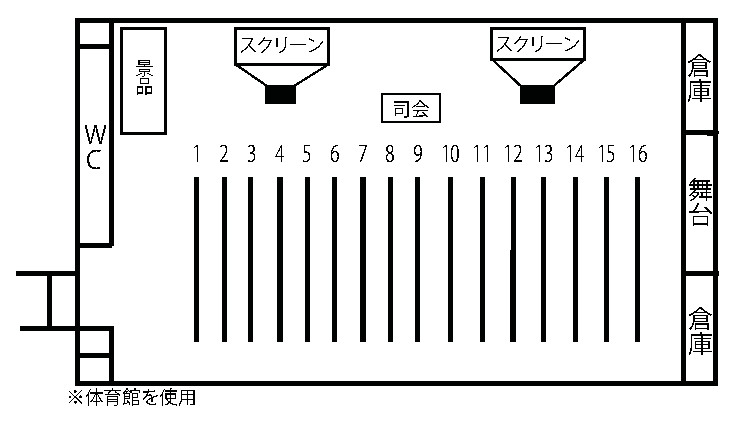
\includegraphics[width = 15cm]{./24/hyousyou.eps}
  \caption{退所式}
  \end{center}
\end{figure}

%%%%%%%%%%%%%%%%%%%%%%%%%%%%%%%%%%%%%%%%%%%%%%%%%%%%%%%%%%%%%%%%%%%%%%%%%%%%%%%
%\include{end}
